% Generated by scripts/analyze.mjs — do not hand-edit.
% Preamble: \usepackage{pgfplots}\pgfplotsset{compat=1.18}
% Every figure carries its numbers inline; the CSVs in this directory hold the same data.

\begin{figure}[t]\centering
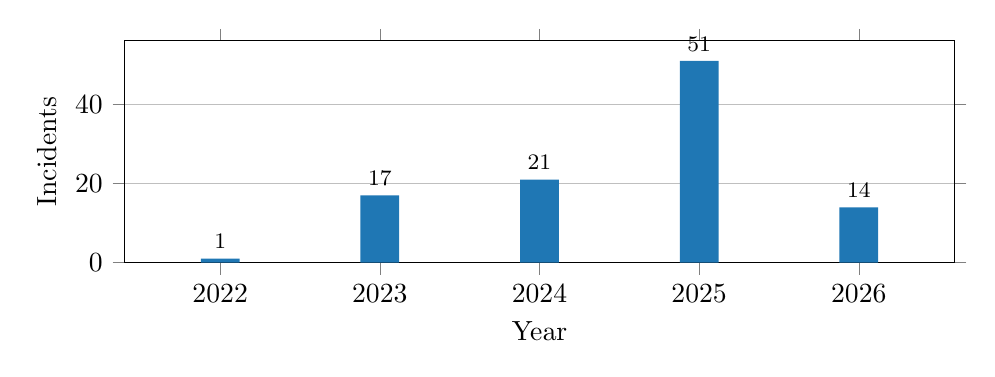
\begin{tikzpicture}
\begin{axis}[width=\columnwidth,height=4.4cm,ybar,bar width=14pt,ymin=0,
  symbolic x coords={2022,2023,2024,2025,2026},xtick=data,
  ylabel={Incidents},xlabel={Year},nodes near coords,every node near coord/.append style={font=\footnotesize},
  enlarge x limits=0.15,ymajorgrids,tick align=outside]
\addplot[fill={rgb,255:red,31;green,119;blue,180},draw=none] coordinates {(2022,1) (2023,17) (2024,21) (2025,51) (2026,14)};
\end{axis}
\end{tikzpicture}
\caption{Documented promptware incidents per year (2026 partial).}\label{fig:per-year}
\end{figure}

\begin{figure}[t]\centering
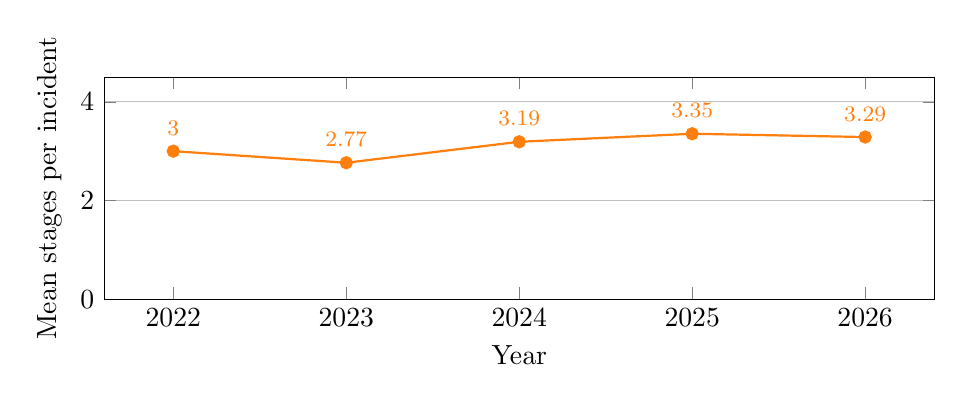
\begin{tikzpicture}
\begin{axis}[width=\columnwidth,height=4.4cm,ymin=0,ymax=4.5,
  symbolic x coords={2022,2023,2024,2025,2026},xtick=data,
  ylabel={Mean stages per incident},xlabel={Year},ymajorgrids,
  nodes near coords={\footnotesize\pgfmathprintnumber[fixed,precision=2]{\pgfplotspointmeta}},
  every node near coord/.append style={yshift=2pt}]
\addplot[mark=*,thick,color={rgb,255:red,255;green,127;blue,14}] coordinates {(2022,3.000) (2023,2.765) (2024,3.190) (2025,3.353) (2026,3.286)};
\end{axis}
\end{tikzpicture}
\caption{Mean kill-chain depth per year. Per-year $n$: 2022: 1, 2023: 17, 2024: 21, 2025: 51, 2026: 14.}\label{fig:mean-stages}
\end{figure}

\begin{figure}[t]\centering
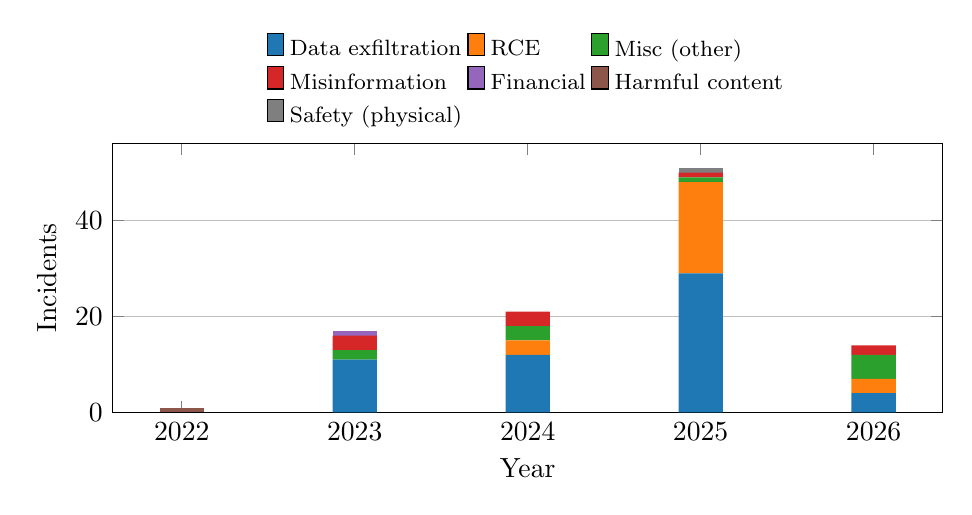
\begin{tikzpicture}
\begin{axis}[width=\columnwidth,height=5cm,ybar stacked,bar width=16pt,ymin=0,
  symbolic x coords={2022,2023,2024,2025,2026},xtick=data,
  ylabel={Incidents},xlabel={Year},ymajorgrids,
  legend style={font=\footnotesize,at={(0.5,1.02)},anchor=south,legend columns=3,draw=none},
  legend cell align=left]
\addplot[fill={rgb,255:red,31;green,119;blue,180},draw=none] coordinates {(2022,0) (2023,11) (2024,12) (2025,29) (2026,4)};
\addlegendentry{Data exfiltration}
\addplot[fill={rgb,255:red,255;green,127;blue,14},draw=none] coordinates {(2022,0) (2023,0) (2024,3) (2025,19) (2026,3)};
\addlegendentry{RCE}
\addplot[fill={rgb,255:red,44;green,160;blue,44},draw=none] coordinates {(2022,0) (2023,2) (2024,3) (2025,1) (2026,5)};
\addlegendentry{Misc (other)}
\addplot[fill={rgb,255:red,214;green,39;blue,40},draw=none] coordinates {(2022,0) (2023,3) (2024,3) (2025,1) (2026,2)};
\addlegendentry{Misinformation}
\addplot[fill={rgb,255:red,148;green,103;blue,189},draw=none] coordinates {(2022,0) (2023,1) (2024,0) (2025,0) (2026,0)};
\addlegendentry{Financial}
\addplot[fill={rgb,255:red,140;green,86;blue,75},draw=none] coordinates {(2022,1) (2023,0) (2024,0) (2025,0) (2026,0)};
\addlegendentry{Harmful content}
\addplot[fill={rgb,255:red,127;green,127;blue,127},draw=none] coordinates {(2022,0) (2023,0) (2024,0) (2025,1) (2026,0)};
\addlegendentry{Safety (physical)}
\end{axis}
\end{tikzpicture}
\caption{Action on objective by year.}\label{fig:outcome-year}
\end{figure}

\begin{figure}[t]\centering
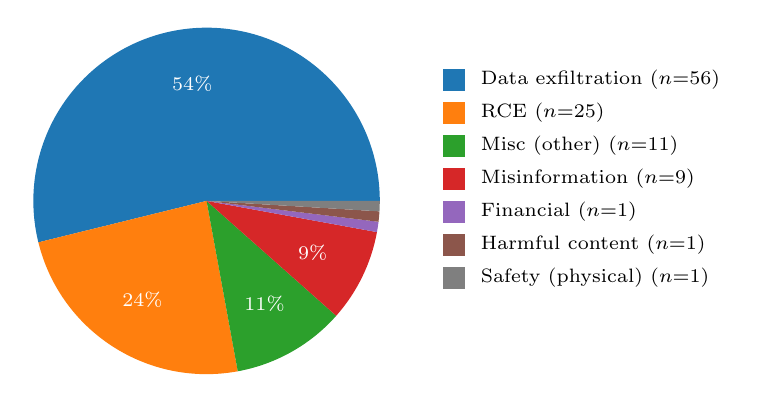
\begin{tikzpicture}
\fill[color={rgb,255:red,31;green,119;blue,180}] (0,0) -- (0.00:2.2) arc (0.00:193.85:2.2) -- cycle;
\node[font=\scriptsize,white] at (96.92:1.5) {54\%};
\fill[color={rgb,255:red,255;green,127;blue,14}] (0,0) -- (193.85:2.2) arc (193.85:280.38:2.2) -- cycle;
\node[font=\scriptsize,white] at (237.12:1.5) {24\%};
\fill[color={rgb,255:red,44;green,160;blue,44}] (0,0) -- (280.38:2.2) arc (280.38:318.46:2.2) -- cycle;
\node[font=\scriptsize,white] at (299.42:1.5) {11\%};
\fill[color={rgb,255:red,214;green,39;blue,40}] (0,0) -- (318.46:2.2) arc (318.46:349.62:2.2) -- cycle;
\node[font=\scriptsize,white] at (334.04:1.5) {9\%};
\fill[color={rgb,255:red,148;green,103;blue,189}] (0,0) -- (349.62:2.2) arc (349.62:353.08:2.2) -- cycle;
\fill[color={rgb,255:red,140;green,86;blue,75}] (0,0) -- (353.08:2.2) arc (353.08:356.54:2.2) -- cycle;
\fill[color={rgb,255:red,127;green,127;blue,127}] (0,0) -- (356.54:2.2) arc (356.54:360.00:2.2) -- cycle;
\begin{scope}[shift={(3.0,1.4)}]
\fill[color={rgb,255:red,31;green,119;blue,180}] (0,0.00) rectangle ++(0.28,0.28);
\node[anchor=west,font=\scriptsize] at (0.36,0.14) {Data exfiltration ($n{=}56$)};
\fill[color={rgb,255:red,255;green,127;blue,14}] (0,-0.42) rectangle ++(0.28,0.28);
\node[anchor=west,font=\scriptsize] at (0.36,-0.28) {RCE ($n{=}25$)};
\fill[color={rgb,255:red,44;green,160;blue,44}] (0,-0.84) rectangle ++(0.28,0.28);
\node[anchor=west,font=\scriptsize] at (0.36,-0.70) {Misc (other) ($n{=}11$)};
\fill[color={rgb,255:red,214;green,39;blue,40}] (0,-1.26) rectangle ++(0.28,0.28);
\node[anchor=west,font=\scriptsize] at (0.36,-1.12) {Misinformation ($n{=}9$)};
\fill[color={rgb,255:red,148;green,103;blue,189}] (0,-1.68) rectangle ++(0.28,0.28);
\node[anchor=west,font=\scriptsize] at (0.36,-1.54) {Financial ($n{=}1$)};
\fill[color={rgb,255:red,140;green,86;blue,75}] (0,-2.10) rectangle ++(0.28,0.28);
\node[anchor=west,font=\scriptsize] at (0.36,-1.96) {Harmful content ($n{=}1$)};
\fill[color={rgb,255:red,127;green,127;blue,127}] (0,-2.52) rectangle ++(0.28,0.28);
\node[anchor=west,font=\scriptsize] at (0.36,-2.38) {Safety (physical) ($n{=}1$)};
\end{scope}
\end{tikzpicture}
\caption{Distribution of action on objective across all 104 incidents.}\label{fig:outcome-pie}
\end{figure}

\begin{figure}[t]\centering
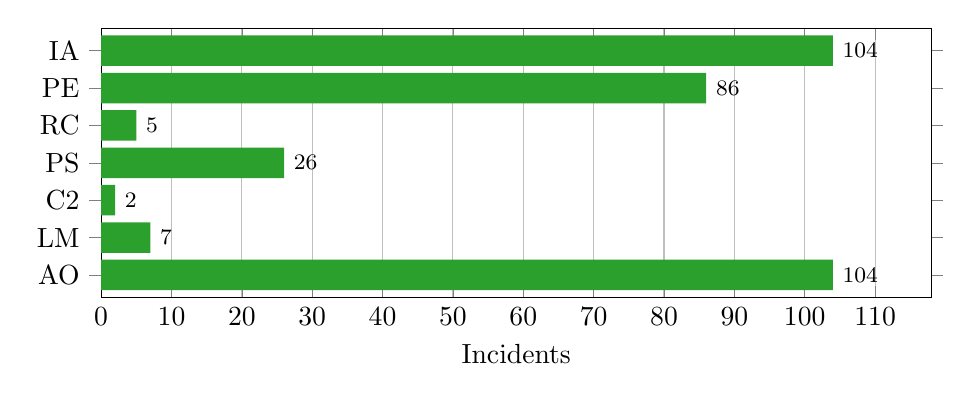
\begin{tikzpicture}
\begin{axis}[width=\columnwidth,height=5cm,xbar,bar width=11pt,xmin=0,xmax=118,
  symbolic y coords={AO,LM,C2,PS,RC,PE,IA},ytick=data,
  xlabel={Incidents},nodes near coords,every node near coord/.append style={font=\footnotesize},
  xmajorgrids]
\addplot[fill={rgb,255:red,44;green,160;blue,44},draw=none] coordinates {(104,AO) (7,LM) (2,C2) (26,PS) (5,RC) (86,PE) (104,IA)};
\end{axis}
\end{tikzpicture}
\caption{Stage prevalence. Initial access and action on objective are universal by construction; reconnaissance, lateral movement, and command and control remain rare.}\label{fig:prevalence}
\end{figure}

\begin{figure}[t]\centering
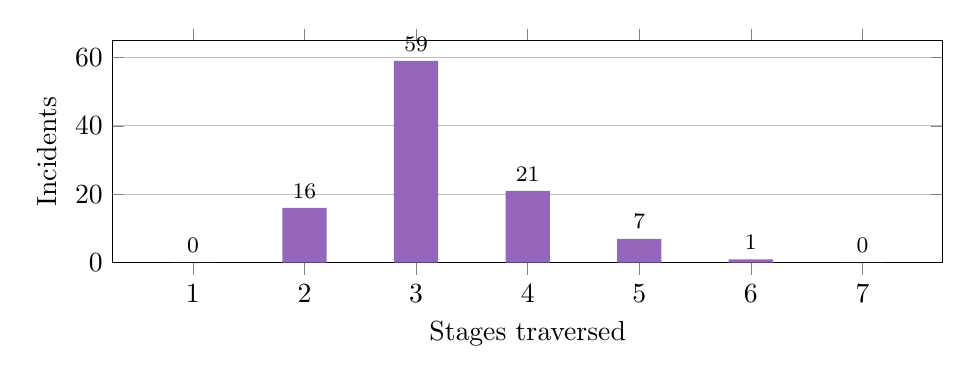
\begin{tikzpicture}
\begin{axis}[width=\columnwidth,height=4.4cm,ybar,bar width=16pt,ymin=0,
  xtick={1,2,3,4,5,6,7},xlabel={Stages traversed},ylabel={Incidents},
  nodes near coords,every node near coord/.append style={font=\footnotesize},ymajorgrids,enlarge x limits=0.12]
\addplot[fill={rgb,255:red,148;green,103;blue,189},draw=none] coordinates {(1,0) (2,16) (3,59) (4,21) (5,7) (6,1) (7,0)};
\end{axis}
\end{tikzpicture}
\caption{Kill-chain depth. 29 of 104 incidents (27.9\%) traverse four or more stages.}\label{fig:chain-length}
\end{figure}

\begin{figure}[t]\centering
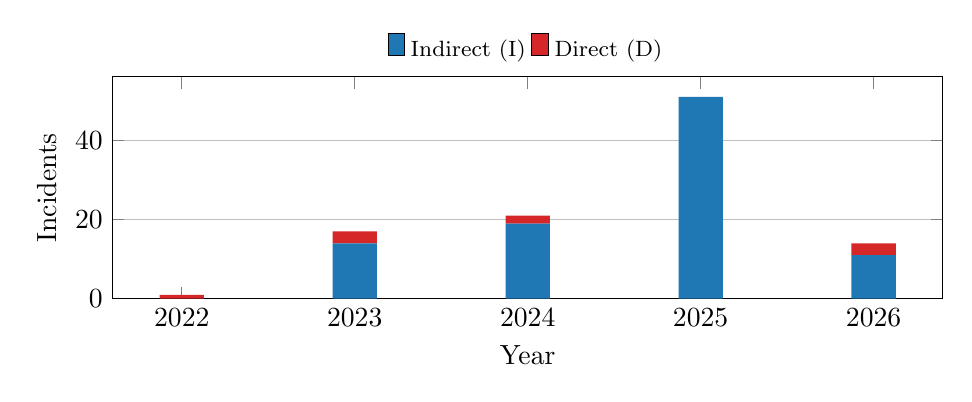
\begin{tikzpicture}
\begin{axis}[width=\columnwidth,height=4.4cm,ybar stacked,bar width=16pt,ymin=0,
  symbolic x coords={2022,2023,2024,2025,2026},xtick=data,ylabel={Incidents},xlabel={Year},ymajorgrids,
  legend style={font=\footnotesize,at={(0.5,1.02)},anchor=south,legend columns=2,draw=none}]
\addplot[fill={rgb,255:red,31;green,119;blue,180},draw=none] coordinates {(2022,0) (2023,14) (2024,19) (2025,51) (2026,11)};\addlegendentry{Indirect (I)}
\addplot[fill={rgb,255:red,214;green,39;blue,40},draw=none] coordinates {(2022,1) (2023,3) (2024,2) (2025,0) (2026,3)};\addlegendentry{Direct (D)}
\end{axis}
\end{tikzpicture}
\caption{Initial access by year. Indirect delivery accounts for 91\% of the corpus.}\label{fig:initial-access}
\end{figure}

\begin{figure}[t]\centering
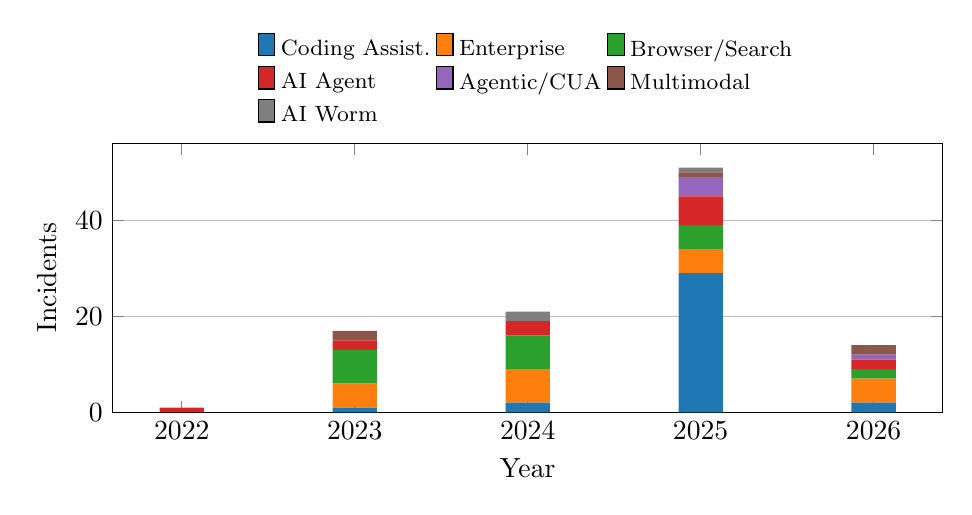
\begin{tikzpicture}
\begin{axis}[width=\columnwidth,height=5cm,ybar stacked,bar width=16pt,ymin=0,
  symbolic x coords={2022,2023,2024,2025,2026},xtick=data,ylabel={Incidents},xlabel={Year},ymajorgrids,
  legend style={font=\footnotesize,at={(0.5,1.02)},anchor=south,legend columns=3,draw=none},legend cell align=left]
\addplot[fill={rgb,255:red,31;green,119;blue,180},draw=none] coordinates {(2022,0) (2023,1) (2024,2) (2025,29) (2026,2)};
\addlegendentry{Coding Assist.}
\addplot[fill={rgb,255:red,255;green,127;blue,14},draw=none] coordinates {(2022,0) (2023,5) (2024,7) (2025,5) (2026,5)};
\addlegendentry{Enterprise}
\addplot[fill={rgb,255:red,44;green,160;blue,44},draw=none] coordinates {(2022,0) (2023,7) (2024,7) (2025,5) (2026,2)};
\addlegendentry{Browser/Search}
\addplot[fill={rgb,255:red,214;green,39;blue,40},draw=none] coordinates {(2022,1) (2023,2) (2024,3) (2025,6) (2026,2)};
\addlegendentry{AI Agent}
\addplot[fill={rgb,255:red,148;green,103;blue,189},draw=none] coordinates {(2022,0) (2023,0) (2024,0) (2025,4) (2026,1)};
\addlegendentry{Agentic/CUA}
\addplot[fill={rgb,255:red,140;green,86;blue,75},draw=none] coordinates {(2022,0) (2023,2) (2024,0) (2025,1) (2026,2)};
\addlegendentry{Multimodal}
\addplot[fill={rgb,255:red,127;green,127;blue,127},draw=none] coordinates {(2022,0) (2023,0) (2024,2) (2025,1) (2026,0)};
\addlegendentry{AI Worm}
\end{axis}
\end{tikzpicture}
\caption{Targeted application category by year.}\label{fig:category-year}
\end{figure}

\begin{figure}[t]\centering
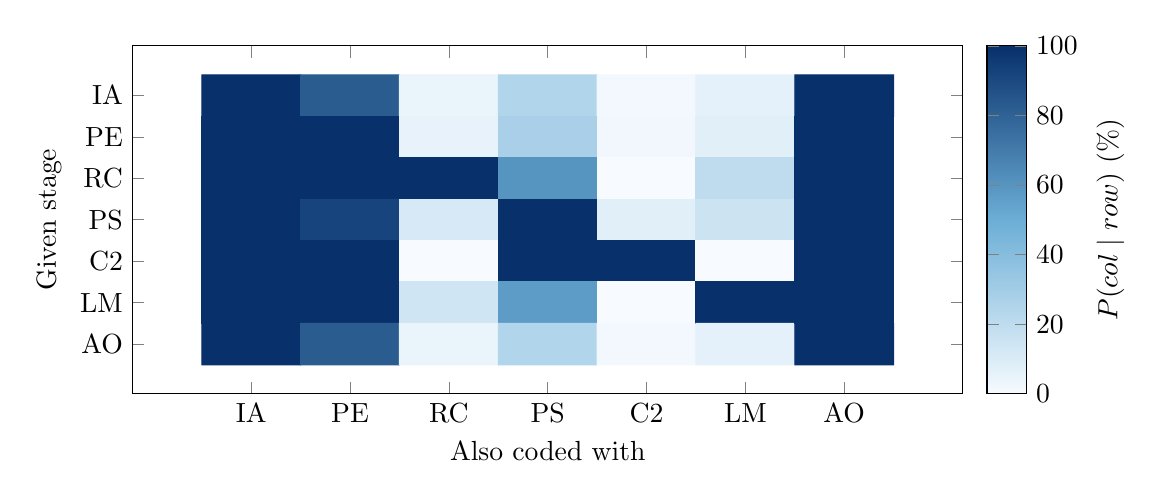
\begin{tikzpicture}
\begin{axis}[width=\columnwidth,height=6cm,
  colormap={paperblues}{rgb255(0cm)=(247,251,255) rgb255(1cm)=(107,174,214) rgb255(2cm)=(8,48,107)},
  colorbar,point meta min=0,point meta max=100,
  xtick={0,...,6},xticklabels={IA,PE,RC,PS,C2,LM,AO},
  ytick={0,...,6},yticklabels={AO,LM,C2,PS,RC,PE,IA},
  xlabel={Also coded with},ylabel={Given stage},
  colorbar style={ylabel={$P(\text{col}\mid\text{row})$ (\%)}}]
\addplot[matrix plot*,mesh/cols=7,point meta=explicit] table[meta index=2] {
x y meta
0 6 100.0
1 6 82.7
2 6 4.8
3 6 25.0
4 6 1.9
5 6 6.7
6 6 100.0
0 5 100.0
1 5 100.0
2 5 5.8
3 5 27.9
4 5 2.3
5 5 8.1
6 5 100.0
0 4 100.0
1 4 100.0
2 4 100.0
3 4 60.0
4 4 0.0
5 4 20.0
6 4 100.0
0 3 100.0
1 3 92.3
2 3 11.5
3 3 100.0
4 3 7.7
5 3 15.4
6 3 100.0
0 2 100.0
1 2 100.0
2 2 0.0
3 2 100.0
4 2 100.0
5 2 0.0
6 2 100.0
0 1 100.0
1 1 100.0
2 1 14.3
3 1 57.1
4 1 0.0
5 1 100.0
6 1 100.0
0 0 100.0
1 0 82.7
2 0 4.8
3 0 25.0
4 0 1.9
5 0 6.7
6 0 100.0
};
\end{axis}
\end{tikzpicture}
\caption{Stage co-occurrence: of incidents coded with the row stage, the percentage also coded with the column stage.}\label{fig:cooccurrence}
\end{figure}

\begin{figure}[t]\centering
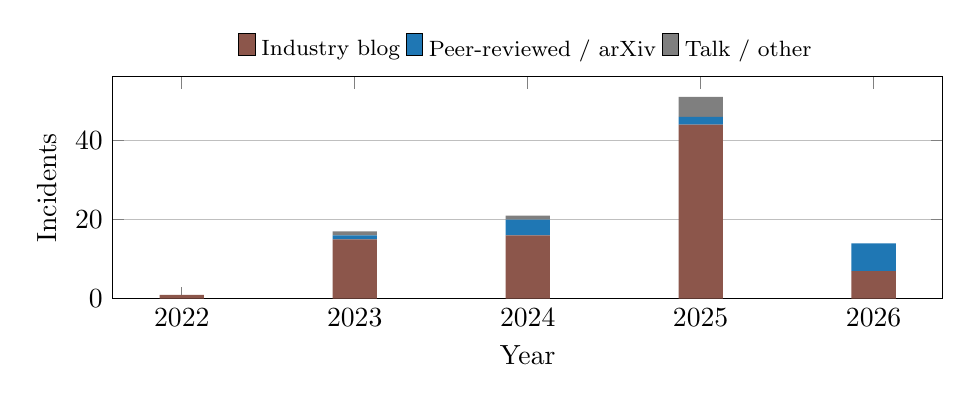
\begin{tikzpicture}
\begin{axis}[width=\columnwidth,height=4.4cm,ybar stacked,bar width=16pt,ymin=0,
  symbolic x coords={2022,2023,2024,2025,2026},xtick=data,ylabel={Incidents},xlabel={Year},ymajorgrids,
  legend style={font=\footnotesize,at={(0.5,1.02)},anchor=south,legend columns=3,draw=none}]
\addplot[fill={rgb,255:red,140;green,86;blue,75},draw=none] coordinates {(2022,1) (2023,15) (2024,16) (2025,44) (2026,7)};\addlegendentry{Industry blog}
\addplot[fill={rgb,255:red,31;green,119;blue,180},draw=none] coordinates {(2022,0) (2023,1) (2024,4) (2025,2) (2026,7)};\addlegendentry{Peer-reviewed / arXiv}
\addplot[fill={rgb,255:red,127;green,127;blue,127},draw=none] coordinates {(2022,0) (2023,1) (2024,1) (2025,5) (2026,0)};\addlegendentry{Talk / other}
\end{axis}
\end{tikzpicture}
\caption{Source provenance by year: the corpus is industry-led, with academic publication trailing.}\label{fig:provenance}
\end{figure}
